\section{Introduction}
\label{sec:introduction}

Distributional analysis of national legislation increasingly demands
answers at geographies the underlying surveys were never designed to
support. A bill's incidence varies with joint characteristics ---
wealth and program participation, tipped occupation and family
structure, itemization and state of residence --- that no single
public-use survey observes together, and legislators consume results
at the grain of states and congressional districts, where survey
samples thin to a few hundred households. The microdata problem is
therefore twofold. First, \emph{fill}: attach the variables a policy
model needs but the base survey lacks, from donor surveys and
administrative sources, without distorting the joints that make
simulation meaningful. Second, \emph{represent}: weight the enhanced
file so it reproduces administrative aggregates across nested
geographies --- national, state, and district --- while remaining
small enough to simulate interactively.

This paper presents the two-stage pipeline that answers both demands
in \populace{},\footnote{\populace{} was first released under the name Populace; frozen artifact, release, and schema identifiers retain the legacy \texttt{populace-}/\texttt{ledger-} prefixes, and this paper cites those identifiers verbatim.} \policyengine{}'s open-source microdata stack
(\autoref{fig:pipeline}). Stage one is a weighted, regime-gated,
sequentially chained quantile-regression-forest imputation operator.
Stage two is a target-informed record-selection and calibration step:
$L_0$-regularized gates, in the Hard Concrete relaxation, jointly
choose which enhanced records to retain and assign each a positive
weight, driven by tens of thousands of administrative calibration
targets rather than by random subsampling.

\begin{figure}[t]
  \centering
  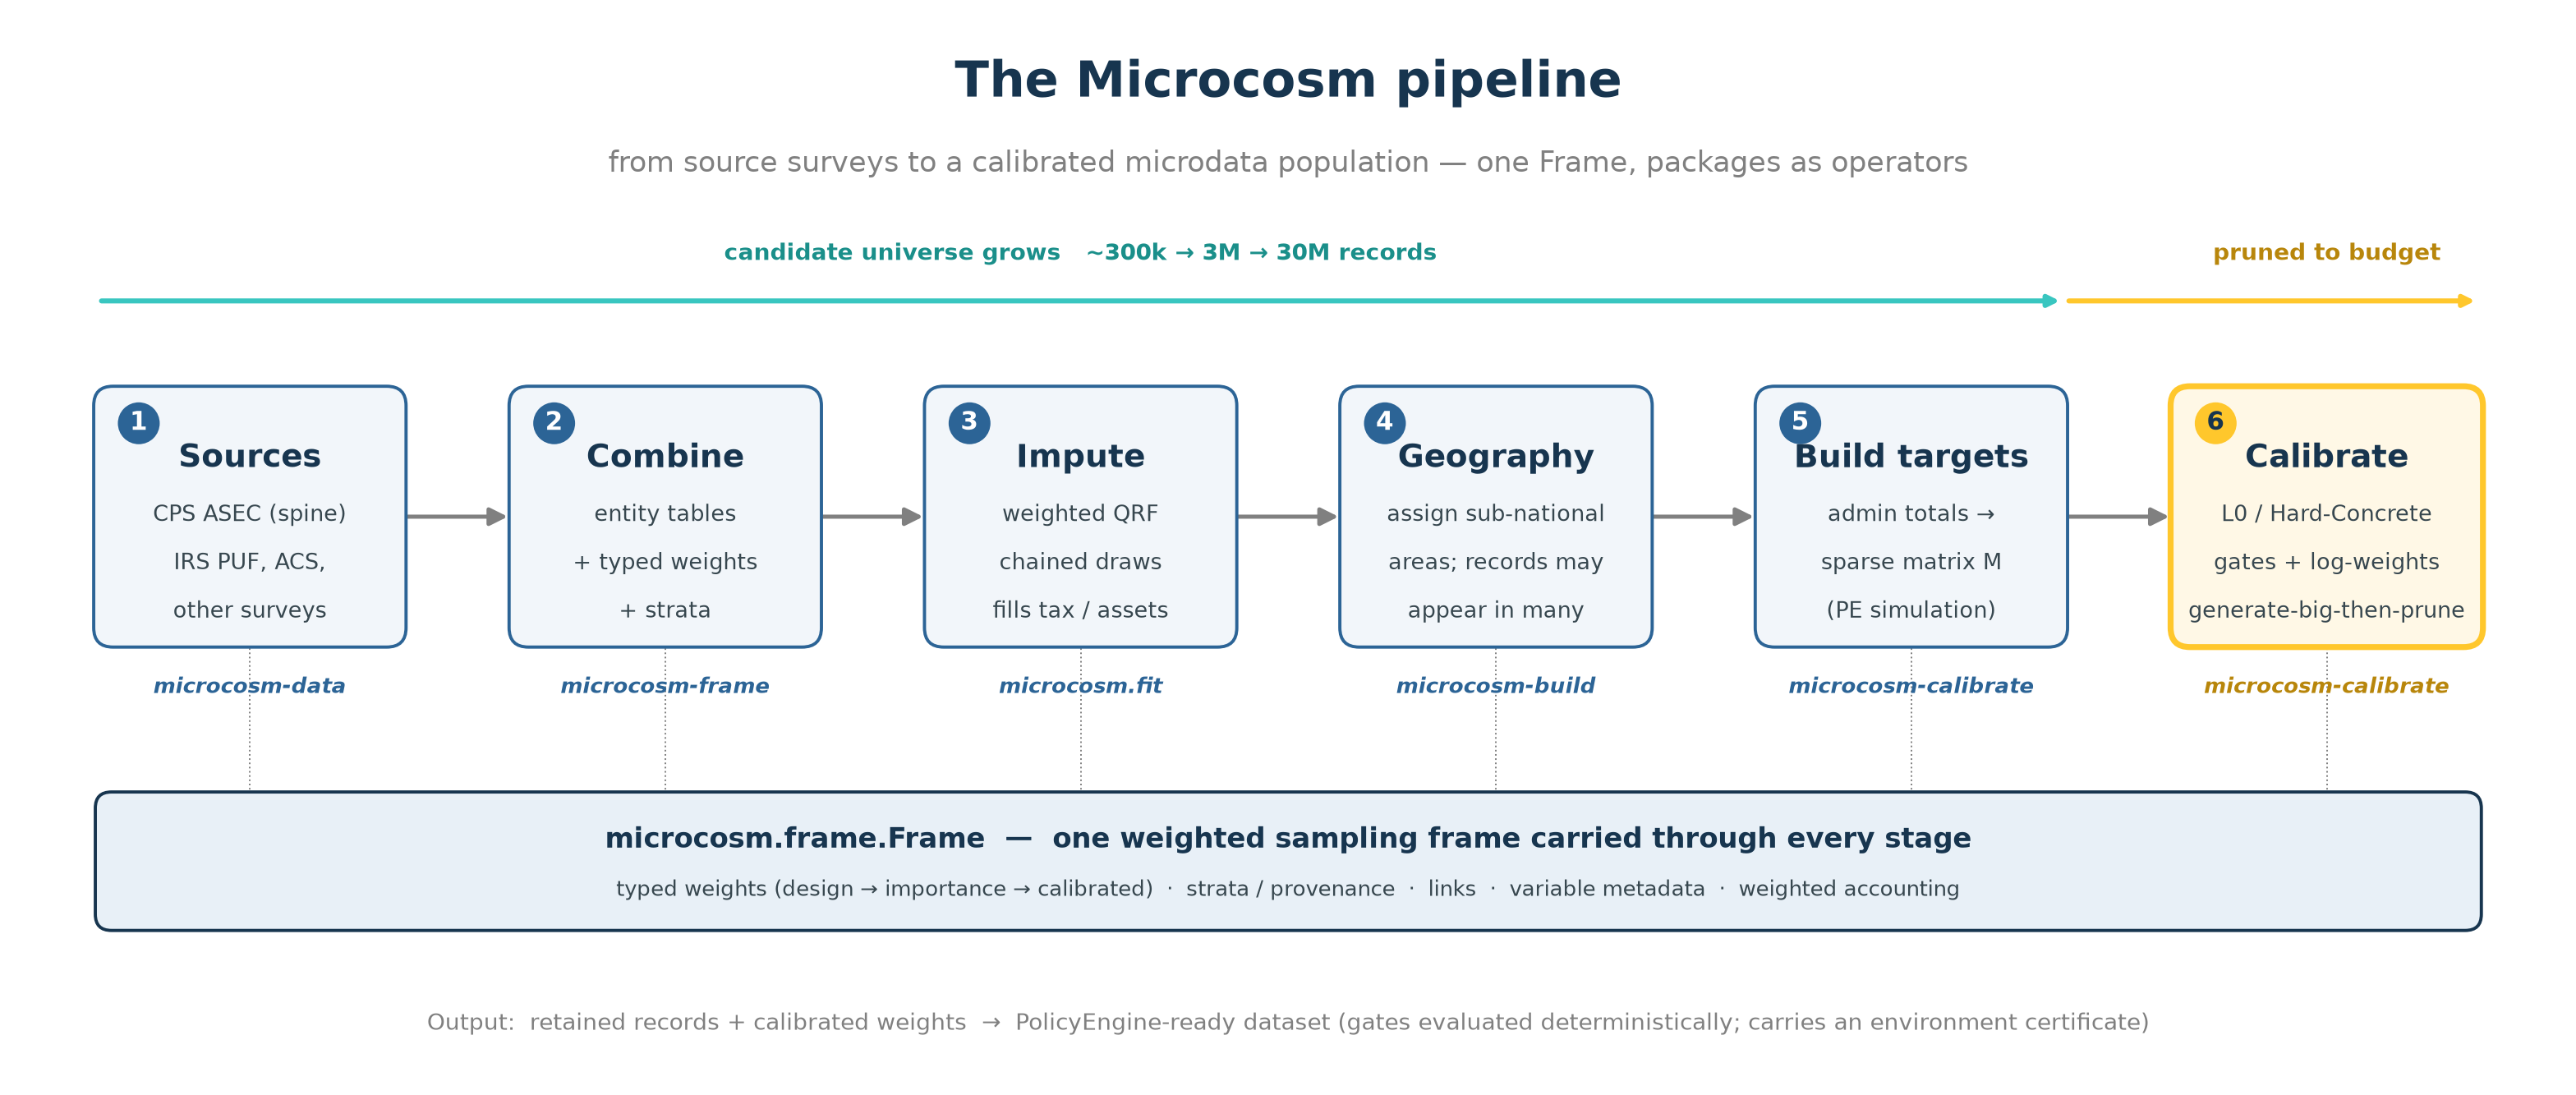
\includegraphics[width=0.92\textwidth]{figures/populace_pipeline}
  \caption{The two-stage pipeline. In the configuration used here,
  source surveys are loaded and combined into a weighted frame; stage
  one imputes missing variables; and stage two assigns geography,
  constructs administrative calibration targets, and applies
  target-informed $L_0$ selection and calibration to produce a sparse,
  simulable, geography-consistent release.}
  \label{fig:pipeline}
\end{figure}

Three design commitments run through both stages. \emph{Respect the
design}: imputation models fit to survey records while ignoring their
weights bias imputed conditionals toward the sample rather than the
population, and the damage concentrates exactly where policy analysis
is most sensitive --- the tails. \emph{Make evaluation match the
estimand}: we score candidate files in a population-view harness ---
one latent population observed through survey views, with strictly
proper joint scores, a coverage axis invariant to candidate
reweighting, classifier two-sample tests, and an uncapped tail block
--- after showing that headline joint-geometry metrics certify files
whose top percentile is wrong by a factor of two. \emph{Let the
targets choose the records}: reduction to a simulable support is
itself an estimation step, and selection informed by the calibration
targets dominates random subsampling at equal record count.

The empirical sections establish, for stage one, that weighting where
the survey design is informative is first-order (the identical
estimator fit unweighted is six times worse on within-donor net-worth
fit, with an imputed 99th percentile 1.9 to 2.3 times the holdout's);
that regime gating carries zero-inflated income components; and that
sequential chaining binds at scale, where independently fitted
balance-sheet components cost 5.8 points of two-sample AUC against a
classifier that detects balance sheets failing to add up. For stage
two, on the full United States target surface --- 32{,}633
materialized targets, including 24{,}340 congressional-district
targets, over 337{,}704 candidate households --- gates select a
57{,}240-record support whose post-selection refit reaches a 4.74\%
capped calibration loss, against 5.07\% for dense calibration of the
full candidate file and 7.55\% for random subsampling refit the same
way. The operative recipe is specific: use the gates to choose the
support, then refit publication weights on it.

The pipeline is not a proposal but a deployed system. The
57{,}240-record support produced by stage two ships as the certified
\populace{} United States release, distributed with pinned model and
data versions through \texttt{policyengine.py}; a companion paper
\citep{ghenis2026obbba} consumes it for provision-level incidence
analysis of the One Big Beautiful Bill Act at national, state, and
congressional-district level, and \autoref{sec:application} reports
what that deployment reveals about the value of target-informed
selection --- including a direct comparison against assignment-only
district weights whose tails collapse into artifacts.

The paper proceeds in two parts.
Sections~\ref{imp:sec:background}--\ref{imp:sec:results} present the
imputation stage: background, experimental design, the estimator, and
results under the population-view harness.
Sections~\ref{sp:sec:background}--\ref{sp:sec:results} present the
selection-and-calibration stage: background, the target surface, the
$L_0$ method, and results. \autoref{sec:application} reports the
deployed application, and \autoref{sec:discussion} and
\autoref{sec:conclusion} discuss limitations and conclude.
